\documentclass{article}
\usepackage[utf8]{inputenc}
\usepackage[frenchb]{babel}
\usepackage{graphicx}

\title{STB : Amélioration de la gestion des demandes en flux des utilisateurs}

\author{Juan PIRON}
\date{08 June 2017}

\begin{document}

\maketitle
\section{Objet du document}
Cette spécification définit les exigences relatives à une étude de la gestion en configuration des demandes de flux PGL via le logiciel CAPIRCA. Le besoin fonctionnel ayant étaient exprimés autour de 3 points :
1/ adapter CAPIRCA pour la génération d’accès-liste ASA (similaires à celles des routeurs cisco).
2/ Mettre en place un mécanisme de génération des règles et de leur gestion en configuration à partir des demandes de flux utilisateurs. 
3/ adapter les règles existant pour les injecter dans le système CAPIRCA.

\maketitle
\section{Spécifications techniques actuelles}

\maketitle
\section{Présentation générale de CAPIRCA}

Capirca est un outil conçu pour utiliser des définitions communes des réseaux, des services et des fichiers de règles (politiques) de haut niveau pour faciliter le développement et la manipulation des listes de contrôle d'accès réseau (ACL) pour diverses plates-formes. Il a été développé par Google pour un usage interne et est désormais open source.
Capirca simplifie le développement et la maintenance des filtres réseaux larges et complexes grâce à un seul et simple langage. Il fournit donc un langage de haut niveau facile à utiliser pour la définition des règles de sécurité réseau. Il permet la compilation des règles de sécurité en des filtres réseaux qui peuvent être appliqués à une variété de cibles (Cisco, Juniper, Iptables …).

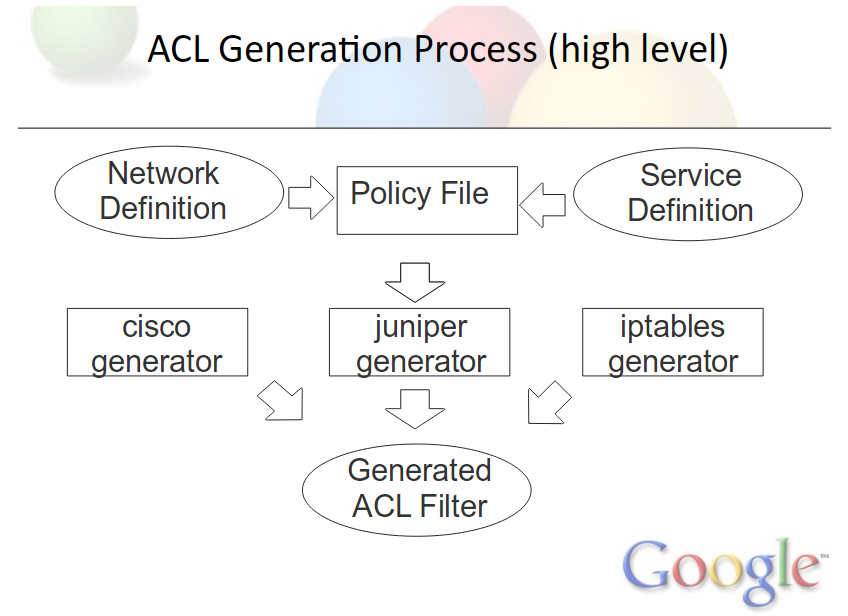
\includegraphics[scale=0.4]{capirca.png}

\maketitle
\section{Spécifications techniques envisagées}

\maketitle
\subsection{Adapter Capirca pour la génération d’accès-list Cisco ASA}

Capirca et constitué de plusieurs "generator", il y a du Cisco, de l’iptables etc. Après des aports de diverses sources Capirca n’a fait que s’enrichir avec le temps. Il faut savoir en effet que Capirca et disponible en open source sur git et toute contribution et la bienvenue. Il s’avère que l’une des dernières contributions est l’ajout du « generator » ciscoasa par Antonio Ceseracciu. Or les accès listes des routeurs PGLs sont du type Cisco ASA v9.1. Cela répond au besoin.

\maketitle
\subsection{Mettre en place un mécanisme de génération des règles et de leur gestion en configuration à partir des demandes de flux utilisateurs}

La solution envisagée ici est la création d’un "serveur" git, plus précisément Gobs. L’avantage de Gobs résidant dans l’existence d’une interface web qui permettrait une gestion plus facile et intuitive des différentes ACLs. Tout cela bien sûr est en open source. Capirca sera placé sur un remote repository, il suffira simplement de creer la policie ou de la modifier et de lancer le script python, et par la suite de faire git add, commit et push. Les polices (langage de haut niveau) seront présentes dans le répertoire capirca/policies/pol et les filtres (ACLs) dans le répertoire capirca/filters. 

\maketitle
\subsection{Adapter les règles existant pour les injecter dans le système CAPIRCA}

En ce qui concerne les règles préexistantes sur les routeurs PGLs les injecters dans le système CAPIRCA revient à réécrire leurs polices. Pour cela il serait possible de créer un script python ou Bash. Mais il s’avère que la manière brute d’écrire les différentes règles (répondant à une demande de flux utilisateur) se présente sous la forme d’un simple fichier CSV. Il paraît donc intéressant de créer un script qui produirait en sortie un fichier en langage de haut niveau. En d’autres termes crée le Generator du langage de haut niveau de capirca.

Pour résumer la solution technique proposée voire le schéma ci-dessous ;

\centerline{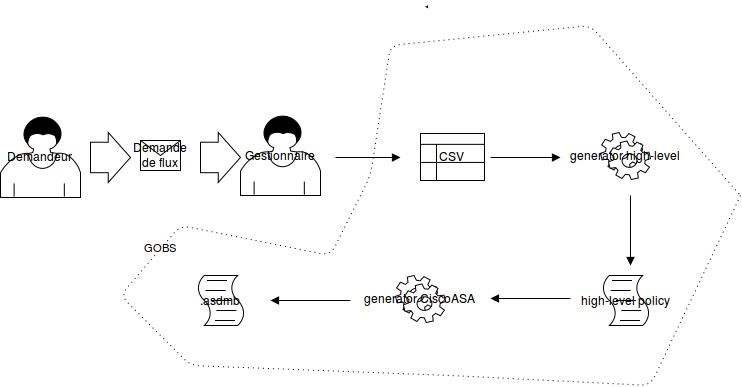
\includegraphics[scale=0.4]{spec.png}}

Par la suite il pourrait être intéressant d'ajouter l'outil de "push" multi-plateform développé par Ryan Shea, LdPush. Cela faciliterait la mise à jour des différentes plateformes avec les nouvelles ACLs.
\end{document}
